
\documentclass[table]{beamer}
\usepackage{etex}
\usetheme{Madrid}


\usepackage[T1]{fontenc}
\usepackage[utf8]{inputenc}
\usepackage{graphicx} % Allows including images
\usepackage{tabularx}
\usepackage{tikz}
\usepackage{pgfplots}
\usepackage{color}


\usetikzlibrary{calc, graphs, arrows.meta}
\usepgflibrary{arrows}

\newcommand{\tikzmark}[2]{\tikz[overlay,remember picture,baseline] \node [anchor=base] (#1) {$#2$};}

\newcommand{\DownArrow}[3][]{%
  \begin{tikzpicture}[overlay,remember picture]
    \draw[-latex, thick,#1] ($(#2.north)+(0,1.0cm)$) -- node [right=3pt]{#3} (#2.north);
  \end{tikzpicture}
}

\newcommand{\UpArrow}[3][]{%
  \begin{tikzpicture}[overlay,remember picture]
    \draw[-latex, thick,#1] ($(#2.south)-(0,1.0cm)$) -- node [right=3pt]{#3} (#2.south);
  \end{tikzpicture}
}

\newcommand{\DrawFlag}[2][]{%
    \begin{tikzpicture}[overlay,remember picture]
        \fill[#1] ($(#2.south)-(0,25pt)$) circle (4pt);
    \end{tikzpicture}
}

\newcommand{\CurvedArrow}[3][]{%
  \begin{tikzpicture}[overlay,remember picture]
      \draw[-latex, thick, #1, ->] (#2.south) to [out = 270, in = 90] (#3.north);
  \end{tikzpicture}
}

\newcommand{\CurvedArrowAbove}[3][]{%
  \begin{tikzpicture}[overlay,remember picture]
      \draw[-latex, thick, #1, ->] (#2.north) to [out = 120, in = 60] (#3.north);
  \end{tikzpicture}
}


\usepackage{cancel}
\usepackage{hhline}
\usepackage{booktabs}
\usepackage{array}

\usepackage{nameref}
\makeatletter
\newcommand*{\currentname}{\@currentlabelname}
\makeatother

\newcommand{\green}{\cellcolor{green!20}}
\newcommand{\yellow}{\cellcolor{yellow!40}}
\newcommand{\blue}{\cellcolor{blue!20}}
\newcommand{\gray}{\cellcolor{gray!20}}
\newcommand{\red}{\cellcolor{red!20}}

%----------------------------------------------------------------------------------------
%	TITLE PAGE
%----------------------------------------------------------------------------------------

\title[Algorithms and Data Structures]{Introduction to Algorithms and Data Structures: An example} % The short title appears at the bottom of every slide, the full title is only on the title page

\author[A. Echavarr\'ia \and S. Palacio]{Ana Echavarr\'ia (aechava3@eafit.edu.co) \and\\ Santiago Palacio (spalac24@eafit.edu.co)} % Your name

\institute[EAFIT] % Your institution as it will appear on the bottom of every slide, may be shorthand to save space
{
EAFIT University \\ % Your institution for the title page
\medskip
}
\date{\today} % Date, can be changed to a custom date

\begin{document}
\newcolumntype{C}{>{\centering\arraybackslash}p{3pt}}

\begin{frame}
\titlepage
\end{frame}

\begin{frame}
\frametitle{Overview}
\tableofcontents
\end{frame}

\section{Algorithms overview}
\frame{\tableofcontents[currentsection]}

\begin{frame}
    \begin{description}
        \setlength\itemsep{10pt}
        \item[Naive] Run through the whole array looking for each element. $O(n^2)$ time.
        \item[DP] Remember already seen elements when looking for them. $O(n * k)$ time.
        \item[Counting] Keep an array of the whole range for counters. $O(n)$ time.
        \item[Sorting] Sort the elements and count consecutive numbers. $O(n*\log(n))$ time.
        \item[Tree] Store the elements in a tree and keep the counter at each node. $O(n*\log(n))$ time.
    \end{description}
\end{frame}

\section{Algorithms real time performance}
\frame{\tableofcontents[currentsection]}

\begin{frame}[fragile]

    \begin{center}
    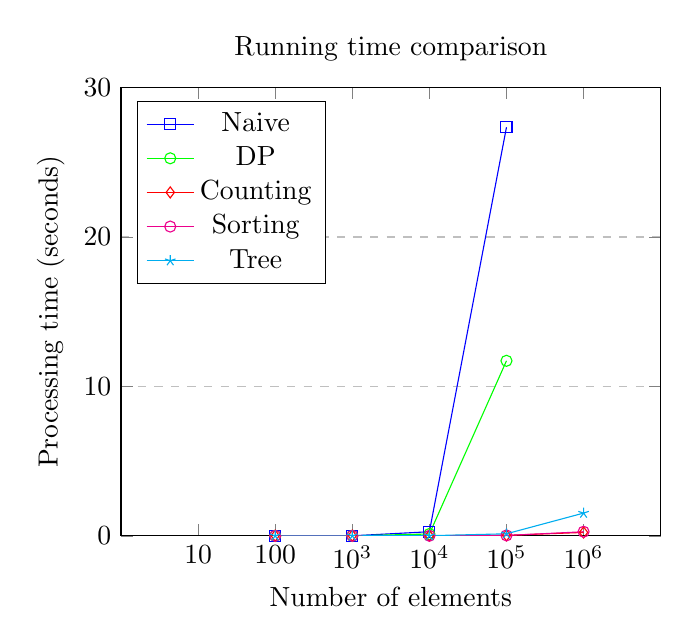
\begin{tikzpicture}
    \begin{axis}[
        title={Running time comparison},
        xlabel={Number of elements},
        ylabel={Processing time (seconds)},
        xmin=0, xmax=7,
        ymin=0, ymax=30,
        xtick={1,2,3,4,5,6},
        xticklabels={10,100,$10^3$,$10^4$,$10^5$, $10^6$},
        legend pos=north west,
        ymajorgrids=true,
        grid style=dashed,
    ]

    \addplot[
        color=blue,
        mark=square,
        ]
        coordinates {
(2,0.0034)
(3,0.0066)
(4,0.2776)
(5,27.346)
    };

    \addplot[
        color=green,
        mark=o,
        ]
        coordinates {
(2,0.0036)
(3,0.0052)
(4,0.1266)
(5,11.716)
    };

    \addplot[
        color=red,
        mark=diamond,
        ]
        coordinates {
(2,0.0136)
(3,0.0142)
(4,0.0162)
(5,0.0364)
(6,0.2318)
    };

    \addplot[
        color=magenta,
        mark=o,
        ]
        coordinates {
(2,0.0036)
(3,0.004)
(4,0.0068)
(5,0.0306)
(6,0.2764)
    };

    \addplot[
        color=cyan,
        mark=star,
        ]
        coordinates {
(2,0.004)
(3,0.0044)
(4,0.0128)
(5,0.1398)
(6,1.5248)
    };

    \legend{Naive,DP,Counting,Sorting,Tree}
    \end{axis}
    \end{tikzpicture}
    \end{center}
\end{frame}

\begin{frame}[fragile]

    \begin{center}
    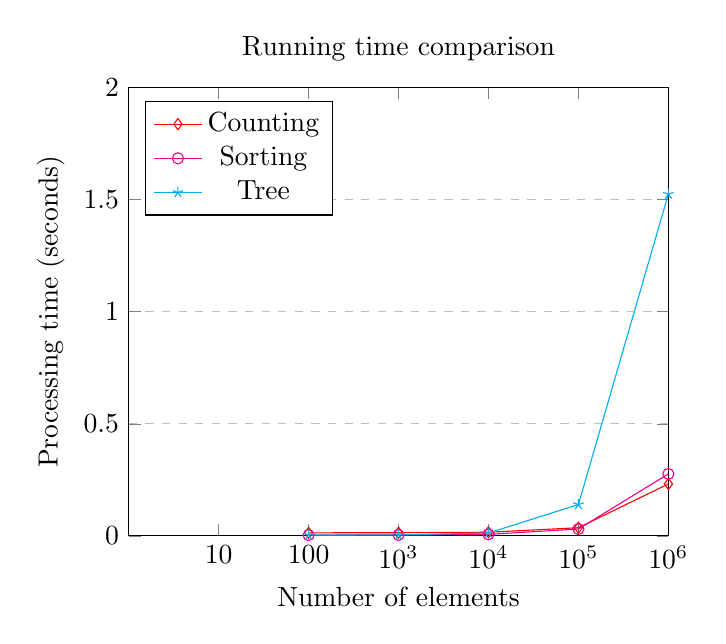
\begin{tikzpicture}
    \begin{axis}[
        title={Running time comparison},
        xlabel={Number of elements},
        ylabel={Processing time (seconds)},
        xmin=0, xmax=6,
        ymin=0, ymax=2,
        xtick={1,2,3,4,5,6},
        xticklabels={10,100,$10^3$,$10^4$,$10^5$, $10^6$},
        legend pos=north west,
        ymajorgrids=true,
        grid style=dashed,
    ]

    \addplot[
        color=red,
        mark=diamond,
        ]
        coordinates {
(2,0.0136)
(3,0.0142)
(4,0.0162)
(5,0.0364)
(6,0.2318)
    };

    \addplot[
        color=magenta,
        mark=o,
        ]
        coordinates {
(2,0.0036)
(3,0.004)
(4,0.0068)
(5,0.0306)
(6,0.2764)
    };

    \addplot[
        color=cyan,
        mark=star,
        ]
        coordinates {
(2,0.004)
(3,0.0044)
(4,0.0128)
(5,0.1398)
(6,1.5248)
    };

    \legend{Counting,Sorting,Tree}
    \end{axis}
    \end{tikzpicture}
    \end{center}
\end{frame}

\section{Algorithms number of operations performance}
\frame{\tableofcontents[currentsection]}

\begin{frame}[fragile]

    \begin{center}
    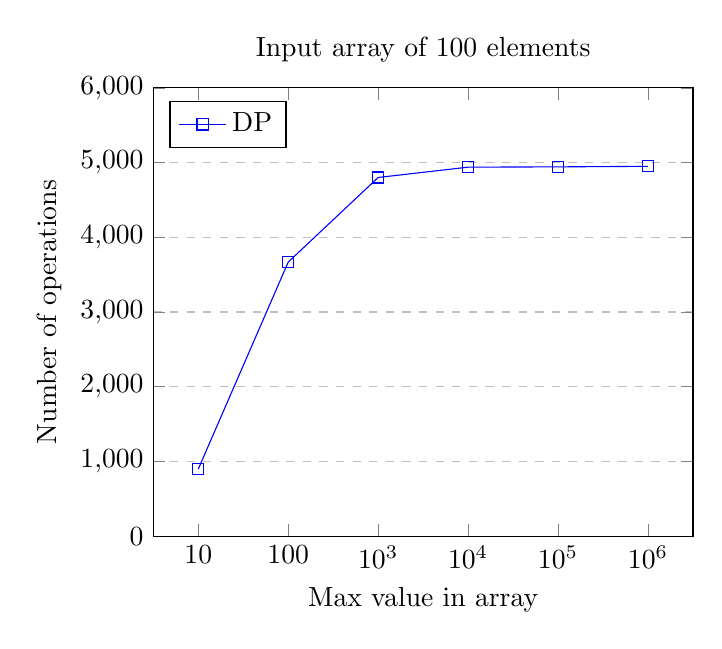
\begin{tikzpicture}
    \begin{axis}[
        title={Input array of $100$ elements},
        xlabel={Max value in array},
        ylabel={Number of operations},
        % xmin=0, xmax=6,
        ymin=0, ymax=6000,
        xtick={1,2,3,4,5,6},
        xticklabels={10,100,$10^3$,$10^4$,$10^5$, $10^6$},
        ytick={0,1000,2000,3000,4000,5000,6000},
        legend pos=north west,
        ymajorgrids=true,
        grid style=dashed,
    ]

    \addplot[
        color=blue,
        mark=square,
        ]
        coordinates {
(1,898.4)
(2,3668.6)
(3,4800.6)
(4,4938.8)
(5,4942.8)
(6,4950.0)
    };


    \legend{DP}
    \end{axis}
    \end{tikzpicture}
    \end{center}
\end{frame}

\begin{frame}[fragile]

    \begin{center}
    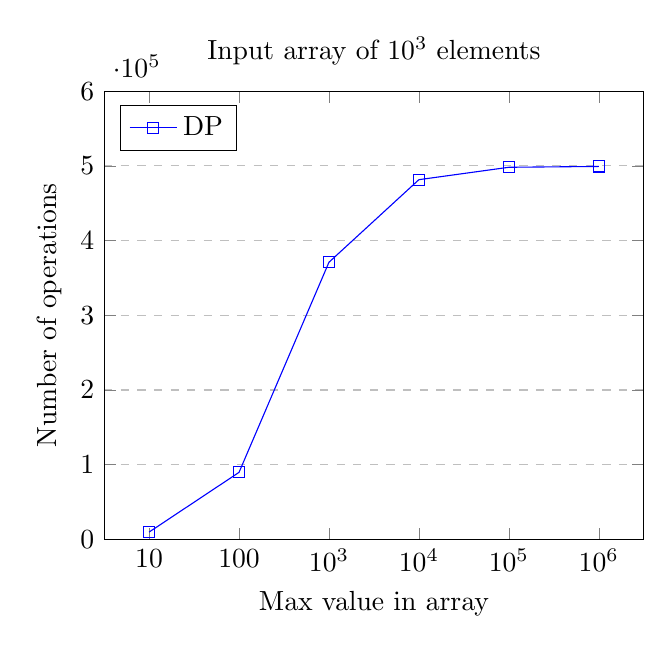
\begin{tikzpicture}
    \begin{axis}[
        title={Input array of $10^3$ elements},
        xlabel={Max value in array},
        ylabel={Number of operations},
        % xmin=0, xmax=6,
        ymin=0, ymax=600000,
        xtick={1,2,3,4,5,6},
        xticklabels={10,100,$10^3$,$10^4$,$10^5$, $10^6$},
        ytick={0,100000,200000,300000,400000,500000,600000},
        legend pos=north west,
        ymajorgrids=true,
        grid style=dashed,
    ]

    \addplot[
        color=blue,
        mark=square,
        ]
        coordinates {
(1,9886.4)
(2,89827.8)
(3,371046.6)
(4,481556.2)
(5,498158.6)
(6,499270)
    };


    \legend{DP}
    \end{axis}
    \end{tikzpicture}
    \end{center}
\end{frame}


\begin{frame}[fragile]

    \begin{center}
    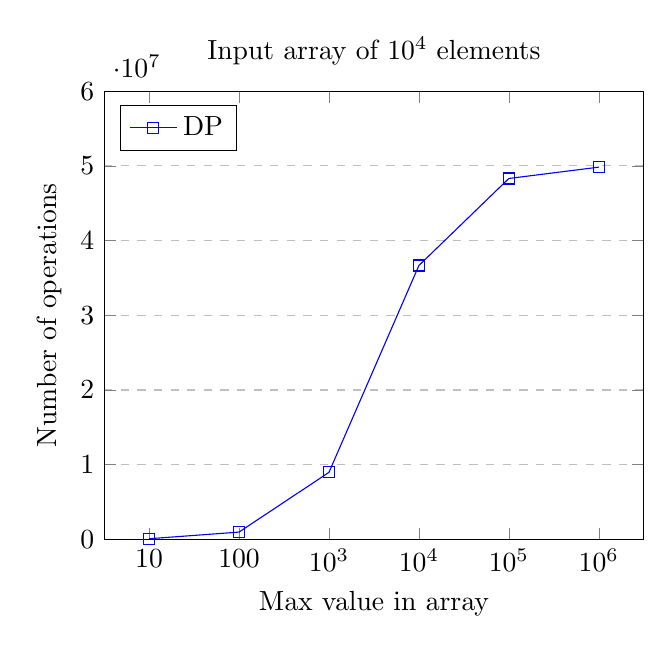
\begin{tikzpicture}
    \begin{axis}[
        title={Input array of $10^4$ elements},
        xlabel={Max value in array},
        ylabel={Number of operations},
        % xmin=0, xmax=6,
        ymin=0, ymax=60000000,
        xtick={1,2,3,4,5,6},
        xticklabels={10,100,$10^3$,$10^4$,$10^5$, $10^6$},
        ytick={0,10000000,20000000,30000000,40000000,50000000,60000000},
        legend pos=north west,
        ymajorgrids=true,
        grid style=dashed,
    ]

    \addplot[
        color=blue,
        mark=square,
        ]
        coordinates {
(1,99895)
(2,989875)
(3,8985523.6)
(4,36667529.2)
(5,48315346)
(6,49833603.8)
    };


    \legend{DP}
    \end{axis}
    \end{tikzpicture}
    \end{center}
\end{frame}


\begin{frame}[fragile]

    \begin{center}
    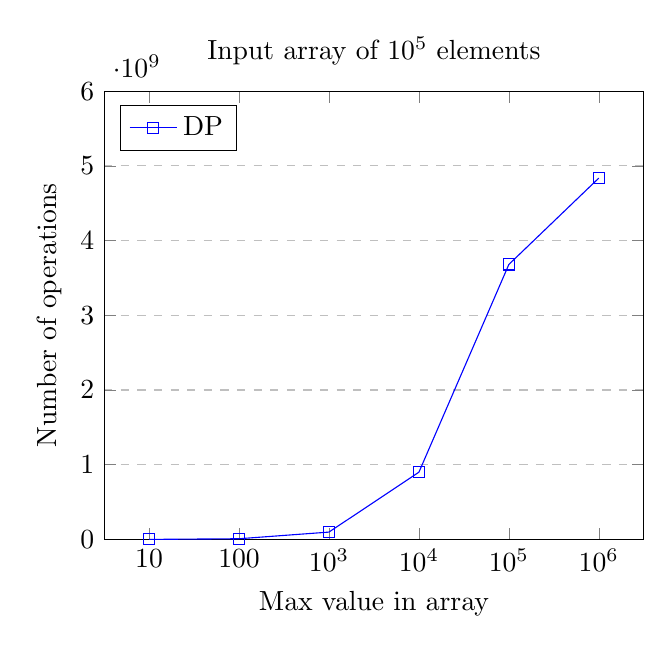
\begin{tikzpicture}
    \begin{axis}[
        title={Input array of $10^5$ elements},
        xlabel={Max value in array},
        ylabel={Number of operations},
        % xmin=0, xmax=6,
        ymin=0, ymax=6000000000,
        xtick={1,2,3,4,5,6},
        xticklabels={10,100,$10^3$,$10^4$,$10^5$, $10^6$},
        ytick={0,1000000000,2000000000,3000000000,4000000000,5000000000,6000000000},
        legend pos=north west,
        ymajorgrids=true,
        grid style=dashed,
    ]

    \addplot[
        color=blue,
        mark=square,
        ]
        coordinates {
(1,999907)
(2,9990194)
(3,98998938.8)
(4,900370571.2)
(5,3680632500)
(6,4836562069)
    };


    \legend{DP}
    \end{axis}
    \end{tikzpicture}
    \end{center}
\end{frame}


\section{Finding elements with a certain frequency}
\frame{\tableofcontents[currentsection]}

\subsection{Finding a majority}
\begin{frame}
    \frametitle{\currentname}
    Given a $stream$ of numbers, find which element, if any, is repeated more than $50\%$ of the time.


    Note: If there is no such element, any output is allowed.
\end{frame}

\begin{frame}
    \frametitle{Sorting solution}
    \begin{itemize}
        \item Sort the complete array.
        \item The element in the middle of the array must be the number we're looking for.
        \item[] \textbf{Disadvantages}
        \item $O(n)$ space, $O(n * log(n))$ time.
    \end{itemize}
\end{frame}

\begin{frame}
    \frametitle{Constant space solution}
    \begin{itemize}
        \item Keep two variables, $count$ and $element$.
        \item Let $count=0$ and $element=null$.
        \item For each element $e$ in the $stream$
        \begin{itemize}
            \item If $e = element$, increase $count$ by $1$.
            \item Otherwise:
            \begin{itemize}
                \item If $count > 0$, decrease it by $1$.
                \item Otherwise, let $element = e$ and $count=1$.
            \end{itemize}
        \end{itemize}

    \end{itemize}
\end{frame}

\begin{frame}
    \frametitle{Example}

    \begin{center}
    	\begin{tabular}{r|C|C|C|C|C|C|C|C|C|}
            \cline{2-10}
    		stream = & \tikzmark{B1}{6\only<3->{\blue}}
    		    & \tikzmark{B2}{3\only<3->{\blue}}
    		    & \tikzmark{B3}{4\only<5->{\red}}
    		    & \tikzmark{B4}{3\only<5->{\red}}
    		    & \tikzmark{B5}{3}
    		    & \tikzmark{B6}{3\only<10->{\green}}
    		    & \tikzmark{B7}{3\only<9->{\yellow}}
    		    & \tikzmark{B8}{2\only<9->{\yellow}}
    		    & \tikzmark{B9}{1\only<10->{\green}}\\
            \cline{2-10}
    	\end{tabular}
    \end{center}

    \hspace{50pt} element = \only<1>{null}\only<2>{6}\only<3>{6}\only<4>{4}\only<5>{4 *}\only<6>{3}\only<7>{3}\only<8>{3}\only<9>{3}\only<10>{3}\\
    \hspace{50pt} count =   \only<1>{0}\only<2>{1}\only<3>{0}\only<4>{1}\only<5>{0}\only<6>{1}\only<7>{2}\only<8>{3}\only<9>{2}\only<10>{1}

    \only<2> {\DownArrow[blue]{B1}{Lookup = 6}}
    \only<3> {\DownArrow[blue]{B2}{Lookup = 3}}
    \only<4> {\DownArrow[blue]{B3}{Lookup = 4}}
    \only<5> {\DownArrow[blue]{B4}{Lookup = 3}}
    \only<6> {\DownArrow[blue]{B5}{Lookup = 3}}
    \only<7> {\DownArrow[blue]{B6}{Lookup = 3}}
    \only<8> {\DownArrow[blue]{B7}{Lookup = 3}}
    \only<9> {\DownArrow[blue]{B8}{Lookup = 2}}
    \only<10> {\DownArrow[blue]{B9}{Lookup = 1}}

\end{frame}

\begin{frame}
    \frametitle{Complexity}
    \begin{itemize}
        \item $O(n)$ time.
        \item $O(\log(\max\{stream\}) + \log(n))$ space.
    \end{itemize}
\end{frame}

\subsection{Generalized problem}
\begin{frame}
    \frametitle{\currentname}
    Given a $stream$ of numbers, find which elements, if any, appear more than $\lfloor n/(k + 1) \rfloor$ times.

    Note: If there are no such elements, any output is allowed.
\end{frame}

\begin{frame}
    \frametitle{$k$ counters soulution}

    \begin{itemize}
        \item Very similar idea as previous algorithm. Instead of a single counter use $k$ counters.
        \item Initialize $k$ counters with value 0.
        \item For every element $e$ in the stream:
        \begin{itemize}
            \item If a counter for $e$ exists, increase its value by one.
            \item If no such counter exists:
                \begin{itemize}
                    \item If there is a counter set to 0, assign it to $e$ with value 1.
                    \item Otherwise decrease all counters by one.
                \end{itemize}
        \end{itemize}
    \end{itemize}
\end{frame}

\begin{frame}
    \frametitle{Example with $k=2$}

    \begin{center}
    	\begin{tabular}{r|C|C|C|C|C|C|C|C|C|C|}
            \cline{2-11}
    		stream =
                & \tikzmark{B1}{1\only<4->{\blue}}
    		    & \tikzmark{B2}{3\only<4->{\blue}}
    		    & \tikzmark{B3}{4\only<4->{\blue}}
    		    & \tikzmark{B4}{3}
    		    & \tikzmark{B5}{3}
    		    & \tikzmark{B6}{1\only<9->{\yellow}}
    		    & \tikzmark{B7}{3\only<9->{\yellow}}
    		    & \tikzmark{B8}{2\only<9->{\yellow}}
    		    & \tikzmark{B9}{1}
                & \tikzmark{B10}{1}\\
            \cline{2-11}
    	\end{tabular}

        \vspace{20pt}
        \begin{tabular}{r|c|c|}
            \cline{2-3}
            element = &
                \only<1>{null}\only<2>{1}\only<3>{1}\only<4>{1}\only<5>{1}\only<6>{1}\only<7>{1}\only<8>{1}\only<9>{1}\only<10>{1}\only<11>{1} &
                \only<1>{null}\only<2>{null}\only<3>{3}\only<4>{3}\only<5>{3}\only<6>{3}\only<7>{3}\only<8>{3}\only<9>{3}\only<10>{3}\only<11>{3}\\
            \cline{2-3}
            count = &
                \only<1>{0}\only<2>{1}\only<3>{1}\only<4>{0}\only<5>{0}\only<6>{0}\only<7>{1}\only<8>{1}\only<9>{0}\only<10>{1}\only<11>{2} &
                \only<1>{0}\only<2>{0}\only<3>{1}\only<4>{0}\only<5>{1}\only<6>{2}\only<7>{2}\only<8>{3}\only<9>{2}\only<10>{2}\only<11>{2}\\
            \cline{2-3}
        \end{tabular}

    \end{center}

    \only<2> {\DownArrow[blue]{B1}{Lookup = 1}}
    \only<3> {\DownArrow[blue]{B2}{Lookup = 3}}
    \only<4> {\DownArrow[blue]{B3}{Lookup = 4}}
    \only<5> {\DownArrow[blue]{B4}{Lookup = 3}}
    \only<6> {\DownArrow[blue]{B5}{Lookup = 3}}
    \only<7> {\DownArrow[blue]{B6}{Lookup = 1}}
    \only<8> {\DownArrow[blue]{B7}{Lookup = 3}}
    \only<9> {\DownArrow[blue]{B8}{Lookup = 2}}
    \only<10> {\DownArrow[blue]{B9}{Lookup = 1}}
    \only<11> {\DownArrow[blue]{B10}{Lookup = 1}}
\end{frame}

\begin{frame}
    \frametitle{Complexity}
    \begin{itemize}
        \item $O(k*n)$ time.
        \item $O(k*(\log(\max\{stream\}) + \log(n)))$ space.
    \end{itemize}
\end{frame}

\end{document}
